
In LLVM, a value is a unique construct – not only does it represent values stored in variables, but it also models a wide range of concepts from constants, global variables, individual instructions, and even basic blocks. In other words, it is one of the foundations of LLVM IR.

The concept of value is especially important for instructions as it directly interacts with values in the IR. Therefore, in this section, we will put them into the same  discussion. We are going to see how values work in LLVM IR and how values are associated with instructions. On top of that, we are going to learn how to create and insert new instructions, as well as how to update them.

To learn how to use values in LLVM IR, we must understand the important theory behind this system, which dictates the behavior and the format of LLVM instructions – the Single Static Assignment (SSA) form.

\subsubsubsection{10.3.1\hspace{0.2cm}Understanding SSA}

SSA is a way of structuring and designing IR to make program analysis and compiler transformation easier to perform. In SSA, a variable (in the IR) will only be assigned a value exactly once. This means that we cannot manipulate a variable like this:

\begin{lstlisting}[style=styleCXX]
// the following code is NOT in SSA form
x = 94;
x = 87; // `x` is assigned the second time, not SSA!
\end{lstlisting}

Although a variable can only be assigned once, it can be used multiple times in arbitrary instructions. For instance, check out the following code:

\begin{lstlisting}[style=styleCXX]
x = 94;
y = x + 4; // first time `x` is used
z = x + 2; // second time `x` is used
\end{lstlisting}

You might be wondering how normal C/C++ code – which is clearly not in SSA form – gets transformed into an SSA form of IR, such as LLVM. While there is a whole class of different algorithms and research papers that answer this question, which we are not going to cover here, most of the simple C/C++ code can be transformed using trivial techniques such as renaming. For instance, let's say we have the following (non-SSA) C code:

\begin{lstlisting}[style=styleCXX]
x = 94;
x = x * y; // `x` is assigned more than once, not SSA!
x = x + 5;
\end{lstlisting}

Here, we can rename x in the first assignment with something like x0 and x on the lefthand side of the second and third assignments with alternative names such as x1 and x2, respectively:

\begin{lstlisting}[style=styleCXX]
x0 = 94;
x1 = x0 * y;
x2 = x1 + 5;
\end{lstlisting}

With these simple measurements, we can obtain the SSA form of our original code with the same behavior.

To have a more comprehensive understanding of SSA, we must change our way of thinking about what instructions look like in a program. In imperative programming languages such as C/C++, we often treat each statement (instruction) as an action. For instance, in the following diagram, on the left-hand side, the first line represents an action that "assigns 94 to variable x" where the second line means "do some multiplication using x and y before storing the result in the x variable":

\hspace*{\fill} \\ %插入空行
\begin{center}
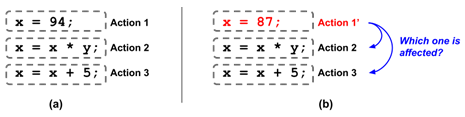
\includegraphics[width=0.9\textwidth]{content/3/chapter10/images/4.png}\\
Figure 10.4 – Thinking instructions as "actions"
\end{center}

These interpretations sound intuitive. However, things get tricky when we make some transformations – which is, of course, a common thing in a compiler – on these instructions. In the preceding diagram, on the right-hand side, when the first instruction becomes x = 87, we don't know if this modification affects other instructions. If it does, we are not sure which one of these gets affected. This information not only tells us whether there are other potential opportunities to optimize, but it is also a crucial factor for the correctness of compiler transformation – after all, no one wants a compiler that will break your code when optimization is enabled. What's worse, let's say we are inspecting the x variable on the right-hand side of Action 3. We are interested in the last few instructions that modify this x. Here, we have no choice but to list all the instructions that have x on their left-hand side (that is, using x as the destination), which is pretty inefficient.

Instead of looking at the action aspect of an instruction, we can focus on the data that's generated by an instruction and get a clear picture of the provenance of each instruction – that is, the region that can be reached by its resulting value. Furthermore, we can easily find out the origins of arbitrary variables/values. The following diagram illustrates this advantage:

\hspace*{\fill} \\ %插入空行
\begin{center}
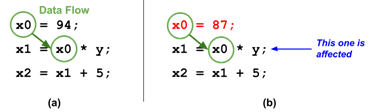
\includegraphics[width=0.9\textwidth]{content/3/chapter10/images/5.png}\\
Figure 10.5 – SSA highlighting the dataflow among instructions
\end{center}

In other words, SSA highlights the dataflow in a program so that the compiler will have an easier time tracking, analyzing, and modify the instructions.

Instructions in LLVM are organized in SSA form. This means we are more interested in the value, or the data flow generated by an instruction, rather than which variable it stores the result in. Since each instruction in LLVM IR can only produce a single result value, an Instruction object – recall that Instruction is the C++ class that represents an instruction in LLVM IR – also represents its result value. To be more specific, the concept of value in LLVM IR is represented by a C++ class called Value. Instruction is one of its child classes. This means that given an Instruction object, we can, of course, cast it to a Value object. That particular Value object is effectively the result of that Instruction:

\begin{lstlisting}[style=styleCXX]
// let's say `I` represents an instruction `x = a + b`
Instruction *I = …;
Value *V = I; // `V` effectively represents the value `x`
\end{lstlisting}

This is one of the most important things to know in order to work with LLVM IR, especially to use most of its APIs.

While the Instruction object represents its own result value, it also has operands that are served as inputs to the instruction. Guess what? We are also using Value objects as operands. For example, let's assume we have the following code:

\begin{lstlisting}[style=styleCXX]
Instruction *BinI = BinaryOperator::Create(Instruction::Add,…);
Instruction *RetI = ReturnInst::Create(…, BinI, …);
\end{lstlisting}

The preceding snippet is basically creating an arithmetic addition instruction (represented by BinaryOperator), whose result value will be the operand of another return instruction. The resulting IR is equivalent to the following C/C++ code:

\begin{lstlisting}[style=styleCXX]
x = a + b;
return x;
\end{lstlisting}

In addition to Instruction, Constant (the C++ class for different kinds of constant values), GlobalVariable (the C++ class for global variables), and BasicBlock are all subclasses of Value. This means that they're also organized in SSA form and that you can use them as the operands for an Instruction.

Now, you know what SSA is and learned what impact it has on the design of LLVM IR. In the next section, we are going to discuss how to modify and update values in LLVM IR.

\subsubsubsection{10.3.2\hspace{0.2cm}Working with values}

SSA makes us focus on the data flow among instructions. Since we have a clear view of how values go from one instruction to the other, it's easy to replace the usage of certain values in an instruction. But how is the concept of "value usage" represented in LLVM? The following diagram shows two important C++ classes that answer this question – User and Use:

\hspace*{\fill} \\ %插入空行
\begin{center}
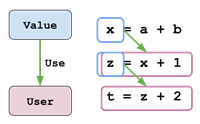
\includegraphics[width=0.9\textwidth]{content/3/chapter10/images/6.png}\\
Figure 10.6 – The relationship between Value, User, and Use
\end{center}

As we can see, User represents the concept of an IR instance (for example, an Instruction) that uses a certain Value. Furthermore, LLVM uses another class, Use, to model the edge between Value and User. Recall that Instruction is a child class of Value – which represents the result that's generated by this instruction. In fact, Instruction is also derived from User, since almost all instructions take at least one operand.

A User might be pointed to by multiple Use instances, which means it uses many Value instances. You can use value\_op\_iterator provided by User to check out each of these Value instances; for example:

\begin{lstlisting}[style=styleCXX]
// `Usr` has the type of `User*`
for (Value *V : Usr->operand_values()) {
	// Working with `V`
}
\end{lstlisting}

Again, operand\_values is just a utility function to generate a value\_op\_iterator range.

Here is an example of why we want to iterate through all the User instances of a Value: imagine we are analyzing a program where one of its Function instances will return sensitive information – let's say, a get\_password function. Our goal is to ensure that whenever get\_password is called within a Function, its returned value (sensitive information) won't be leaked via another function call. For example, we want to detect the following pattern and raise an alarm:

\begin{lstlisting}[style=styleCXX]
void vulnerable() {
	v = get_password();
	…
	bar(v); // WARNING: sensitive information leak to `bar`!
}
\end{lstlisting}

The find\_leackage function takes a CallInst argument – which represents a get\_password function call – and returns any User instance that uses the Value instance that's returned from that get\_password call. 

A Value instance can be used by multiple different User instances. So, similarly, we can iterate through all of them using the following snippet:

\begin{lstlisting}[style=styleCXX]
User *find_leakage(CallInst *GetPWDCall) {
	for (auto *Usr : GetPWDCall->users()) {
		if (isa<CallInst>(Usr)) {
			return Usr;
		}
	}
…
}
\end{lstlisting}

The find\_leackage function takes a CallInst argument – which represents a get\_ password function call – and returns any User instance that uses the Value instance that's returned from that get\_password call.

A Value instance can be used by multiple different User instances. So, similarly, we can iterate through all of them using the following snippet:

\begin{lstlisting}[style=styleCXX]
// `V` has the type of `Value*`
for (User *Usr : V->users()) {
	// Working with `Usr`
}
\end{lstlisting}

With that, you've learned how to inspect the User instance of a Value, or the Value instance that's used by the current User. In addition, when we're developing a compiler transformation, it is pretty common to change the Value instance that's used by a User to another one. LLVM provides some handy utilities to do this.

First, the Value::replaceAllUsesWith method can, as its name suggests, tell all of its User instances to use another Value instead of it. The following diagram illustrates its effect:

\hspace*{\fill} \\ %插入空行
\begin{center}
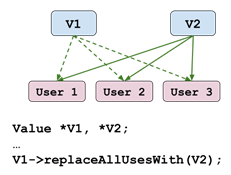
\includegraphics[width=0.9\textwidth]{content/3/chapter10/images/7.png}\\
Figure 10.7 – Effect of Value::replaceAllUsesWith
\end{center}

This method is really useful when you're replacing an Instruction with another Instruction. Using the preceding diagram to explain this, V1 is the original Instruction and V2 is the new one.

Another utility function that does a similar thing is User::replaceUsesOfWith(From,To). This method effectively scans through all of the operands in this User and replaces the usage of a specific Value (the From argument) with another Value (the To argument).

The skills you've learned in this section are some of the most fundamental tools for developing a program transformation in LLVM. In the next section, we will talk about how to create and modify instructions.

\subsubsubsection{10.3.3\hspace{0.2cm}Working with instructions}

Previously, we learned the basics of Value – including its relationship with Instruction – and the way to update Value instances under the framework of SSA. In this section, we are going to learn some more basic knowledge and skills that give you a better understanding of Instruction and help you modify Instruction instances in a correct and efficient way, which is the key to developing a successful compiler optimization.

Here is the list of topics we are going to cover in this section:

\begin{itemize}
\item Casting between different instruction types
\item Inserting a new instruction
\item Replacing an instruction
\item Processing instructions in batches
\end{itemize}

Let's start by looking at different instruction types.

\hspace*{\fill} \\ %插入空行
\noindent
\textbf{Casting between different instruction types}

In the previous section, we learned about a useful utility called InstVisitor. The InstVisitor class helps you determine the underlying class of an Instruction instance. It also saves you the efforts of casting between different instruction types. However, we cannot always rely on InstVisitor for every task that involves type casting between Instruction and its derived classes. More generally speaking, we want a simpler solution for type casting between parent and child classes.

Now, you might be wondering, but C++ already provided this mechanism via the dynamic\_cast directive, right? Here is an example of dynamic\_cast:

\begin{lstlisting}[style=styleCXX]
class Parent {…};
class Child1 : public Parent {…};
class Child2 : public Parent {…};

void foo() {
	Parent *P = new Child1();
	Child1 *C = dynamic_cast<Child1*>(P); // OK
	Child2 *O = dynamic_cast<Child2*>(P); // Error: bails out at
	// runtime
}
\end{lstlisting}

In the foo function used in the preceding code, we can see that in its second line, we can convert P into a Child1 instance because that is its underlying type. On the other hand, we cannot convert P into Child2 – the program will simply crash during runtime if we do so. 

Indeed, dynamic\_cast has the exact functionality we are looking for – more formally speaking, the Runtime Type Info (RTTI) feature – but it also comes with high overhead in terms of runtime performance. What's worse, the default implementation of RTTI in C++ is quite complex, making the resulting program difficult to optimize. Therefore, LLVM disables RTTI by default. Due to this, LLVM came up with its own system of runtime type casting that is much simpler and more efficient. In this section, we are going to talk about how to use it.

LLVM's casting framework provides three functions for dynamic type casting:

\begin{itemize}
\ttfamily
\item isa<T>(val)
\item cast<T>(val)
\item dyn\_cast<T>(val)
\end{itemize}

The first function, isa<T> – pronounced "is-a" – checks if the val pointer type can be cast to a pointer of the T type. Here is an example:

\begin{lstlisting}[style=styleCXX]
// `I` has the type of `Instruction*`
if (isa<BinaryOperator>(I)) {
	// `I` can be casted to `BinaryOperator*`
}
\end{lstlisting}

Note that differently from dynamic\_cast, you don't need to put BinaryOperator* as the template argument in this case – only a type without a pointer qualifier.

The cast<T> function performs the real type casting from (pointer-type) val to a pointer of the T type. Here is an example:

\begin{lstlisting}[style=styleCXX]
// `I` has the type of `Instruction*`
if (isa<BinaryOperator>(I)) {
	BinaryOperator *BinOp = cast<BinaryOperator>(I);
}
\end{lstlisting}

Again, you don't need to put BinaryOperator* as the template argument. Note that if you don't perform type checking using isa<T> before calling cast<T>, the program will just crash during runtime.

The last function, dyn\_cast<T>, is a combination of isa<T> and cast<T>; that is, you perform type casting if applicable. Otherwise, it returns a null. Here is an example:

\begin{lstlisting}[style=styleCXX]
// `I` has the type of `Instruction*`
if (BinaryOperator *BinOp = dyn_cast<BinaryOperator>(I)) {
	// Work with `BinOp`
}
\end{lstlisting}

Here, we can see some neat syntax that combines the variable declaration (of BinOp) with the if statement.

Be aware that none of these APIs can take null as the argument. On the contrary, dyn\_cast\_or\_null<T> doesn't have this limitation. It is basically a dyn\_cast<T> API that accepts null as input.

Now, you know how to check and cast from an arbitrary Instruction instance to its underlying instruction type. Starting from the next section, we are finally going to create and modify some instructions.

\hspace*{\fill} \\ %插入空行
\noindent
\textbf{Inserting a new instruction}

In one of the code examples from the previous Understanding SSA section, we saw a snippet like this:

\begin{lstlisting}[style=styleCXX]
Instruction *BinI = BinaryOperator::Create(…);
Instruction *RetI = ReturnInst::Create(…, BinI, …);
\end{lstlisting}

As suggested by the method's name – Create – we can infer that these two lines created a BinaryOperator and a ReturnInst instruction.

Most of the instruction classes in LLVM provide factory methods – such as Create here – to build a new instance. People are encouraged to use these factory methods versus allocating instruction objects manually via the new keyword or malloc function. LLVM will manage the instruction object's memory for you – once it's been inserted into a BasicBlock. There are several ways to insert a new instruction into a BasicBlock:

\begin{itemize}
\item Factory methods in some instruction classes provide an option to insert the instruction right after it is created. For instance, one of the Create method variants in BinaryOperator allows you to insert it before another instruction after the creation. Here is an example:

\begin{lstlisting}[style=styleCXX]
Instruction *BeforeI = …;
auto *BinOp = BinaryOperator::Create(Opcode, LHS, RHS,
  "new_bin_op", BeforeI);
\end{lstlisting}

In such a case, the instruction represented by BinOp will be placed before the one represented by BeforeI. This method, however, can't be ported across different instruction classes. Not every instruction class has factory methods that provide this feature and even if they do provide them, the API might not be the same.

\item We can use the insertBefore/insertAfter methods provided by the Instruction class to insert a new instruction. Since all instruction classes are subclasses of Instruction, we can use insertBefore or insertAfter to insert the newly created instruction instance before or after another Instruction.
 
\item We can also use the IRBuilder class. IRBuilder is a powerful tool for automating some of the instruction creation and insertion steps. It implements a builder design pattern that can insert new instructions one after another when developers invoke one of its creation methods. Here is an example:

\begin{lstlisting}[style=styleCXX]
// `BB` has the type of `BasicBlock*`
IRBuilder<> Builder(BB /*the insertion point*/);
// insert a new addition instruction at the end of `BB`
auto *AddI = Builder.CreateAdd(LHS, RHS);
// Create a new `ReturnInst`, which returns the result
// of `AddI`, and insert after `AddI`
Builer.CreateRet(AddI);
\end{lstlisting}

First, when we create an IRBuilder instance, we need to designate an insertion point as one of the constructor arguments. This insertion point argument can be a BasicBlock, which means we want to insert a new instruction at the end of BasicBlock; it can also be an Instruction instance, which means that new instructions are going to be inserted before that specific Instruction.

You are encouraged to use IRBuilder over other mechanisms if possible whenever you need to create and insert new instructions in sequential order.

\end{itemize}

With that, you've learned how to create and insert new instructions. Now, let's look at how to replace existing instructions with others.


\hspace*{\fill} \\ %插入空行
\noindent
\textbf{Replacing an instruction}

There are many cases where we will want to replace an existing instruction. For instance, a simple optimizer might replace an arithmetic multiplication instruction with a leftshifting instruction when one of the multiplication's operands is a power-of-two integer constant. In this case, it seems straightforward that we can achieve this by simply changing the operator (the opcode) and one of the operands in the original Instruction. That is not the recommended way to do things, however.

To replace an Instruction in LLVM, you need to create a new Instruction (as the replacement) and reroute all the SSA definitions and usages from the original Instruction to the replacement one. Let's use the power-of-two-multiplication we just saw as an example:

\begin{enumerate}
\item The function we are going to implement is called replacePow2Mul, whose argument is the multiplication instruction to be processed (assuming that we have ensured the multiplication has a constant, power-of-two integer operand). First, we will retrieve the constant integer – represented by the ConstantInt class – operand and convert it into its base-2 logarithm value (via the getLog2 utility function; the exact implementation of getLog2 is left as an exercise for you):

\begin{lstlisting}[style=styleCXX]
void replacePow2Mul(BinaryOperator &Mul) {
	// Find the operand that is a power-of-2 integer
	// constant
	int ConstIdx = isa<ConstantInt>(Mul.getOperand(0))? 0
	  : 1;
	ConstantInt *ShiftAmount = getLog2(Mul.
	  getOperand(ConstIdx));
}
\end{lstlisting}

\item Next, we will create a new left-shifting instruction – represented by the ShlOperator class:

\begin{lstlisting}[style=styleCXX]
void replacePow2Mul(BinaryOperator &Mul) {
	…
	// Get the other operand from the original instruction
	auto *Base = Mul.getOperand(ConstIdx? 0 : 1);
	// Create an instruction representing left-shifting
	IRBuilder<> Builder(&Mul);
	auto *Shl = Builder.CreateShl(Base, ShiftAmount);
}
\end{lstlisting}

\item Finally, before we remove the Mul instruction, we need to tell all the users of the original Mul to use our newly created Shl instead:

\begin{lstlisting}[style=styleCXX]
void replacePow2Mul(BinaryOperator &Mul) {
	…
	// Using `replaceAllUsesWith` to update users of `Mul`
	Mul.replaceAllUsesWith(Shl);
	Mul.eraseFromParent(); // remove the original
	// instruction
}
\end{lstlisting}

Now, all the original users of Mul are using Shl instead. Thus, we can safely remove Mul from the program.

\end{enumerate}

With that, you've learned how to replace an existing Instruction properly. In the final subsection, we are going to talk about some tips for processing multiple instructions in a BasicBlock or a Function.

\hspace*{\fill} \\ %插入空行
\noindent
\textbf{Tips for processing instructions in batches}

So far, we have been learning how to insert, delete, and replace a single Instruction. However, in real-world cases, we usually perform such actions on a sequence of Instruction instances (that are in a BasicBlock, for instance). Let's try to do that by putting what we've learned into a for loop that iterates through all the instructions in a BasicBlock; for instance:

\begin{lstlisting}[style=styleCXX]
// `BB` has the type of `BasicBlock&`
for (Instruction &I : BB) {
	if (auto *BinOp = dyn_cast<BinaryOperator>(&I)) {
		if (isMulWithPowerOf2(BinOp))
		replacePow2Mul(BinOp);
	}
}
\end{lstlisting}

The preceding code used the replacePow2Mul function we just saw in the previous section to replace the multiplications in this BasicBlock with left-shifting instructions if the multiplication fulfills certain criteria. (This is checked by the isMulWithPowerOf2 function. Again, the details of this function have been left as an exercise to you.)

This code looks pretty straightforward but unfortunately, it will crash while running this transformation. What happened here was that the iterator that's used for enumerating Instruction instances in BasicBlock became stale after running our replacePow2Mul. The Instruction iterator is unable to keep updated with the changes that have been applied to the Instruction instances in this BasicBlock. In other words, it's really hard to change the Instruction instances while iterating them at the same time.

The simplest way to solve this problem is to push off the changes:

\begin{lstlisting}[style=styleCXX]
// `BB` has the type of `BasicBlock&`
std::vector<BinaryOperator*> Worklist;
// Only perform the feasibility check
for (auto &I : BB) {
	if (auto *BinOp = dyn_cast<BinaryOperator>(&I)) {
		if (isMulWithPowerOf2(BinOp)) Worklist.push_back(BinOp);
	}
}
// Replace the target instructions at once
for (auto *BinOp : Worklist) {
	replacePow2Mul(BinOp);
}
\end{lstlisting}

The preceding code separates the previous code example into two parts (as two separate for loops). The first for loop is still iterating through all the Instruction instances in BasicBlock. But this time, it only performs the checks (that is, calling isMulWithPowerOf2) without replacing the Instruction instance right away if it passes the checks. Instead, this for loop pushes the candidate Instruction into array storage – a worklist. After finishing the first for loop, the second for loop inspects the worklist and performs the real replacement by calling replacePow2Mul on each worklist item. Since the replacements in the second for loop don't invalidate any iterators, we can finally transform the code without any crashes occurring.

There are, of course, other ways to circumvent the aforementioned iterator problem, but they are mostly complicated and less readable. Using a worklist is the safest and most expressive way to modify instructions in batches.

Value is a first-class construction in LLVM that outlines the data flow among different entities such as instructions. In this section, we introduced how values are represented in LLVM IR and the model of SSA that makes it easier to analyze and transform it. We also learned how to update values in an efficient way and some useful skills for manipulating instructions. This will help build the foundation for you to build more complex and advanced compiler optimizations using LLVM.

In the next section, we will look at a slightly more complicated IR unit – a loop. We are going to learn how loops are represented in LLVM IR and how to work with them.




















